% Template for PLOS Computational Biology
%
% % % % % % % % % % % % % % % % % % % % % %
%
% -- IMPORTANT NOTE --
%
% This template requires the 'plos2015.bst' BibTeX style file.
%
% % % % % % % % % % % % % % % % % % % % % %

\documentclass[10pt,letterpaper]{article}
\usepackage[top=0.85in,left=2.75in,footskip=0.75in]{geometry}

% amsmath and amssymb packages, useful for mathematical formulas and symbols
\usepackage{amsmath,amssymb}

% Use adjustwidth environment for wider text coverage
\usepackage{changepage}

% textcomp package and marvosym package for additional characters
\usepackage{textcomp,marvosym}

% cite package, to clean up citations in the main text. Do not remove.
\usepackage{cite}

% Use nameref to cite supporting information files (see Supporting Information section for more info)
\usepackage{nameref,hyperref}

% line numbers
\usepackage[right]{lineno}

% ligatures disabled
\usepackage{microtype}
\DisableLigatures[f]{encoding = *, family = * }

% color can be used to apply background shading to table cells only
\usepackage[table]{xcolor}

% array package and thick rules for tables
\usepackage{array}

% create "+" rule type for thick vertical lines
\newcolumntype{+}{!{\vrule width 2pt}}

% create \thickcline for thick horizontal lines of variable length
\newlength\savedwidth
\newcommand\thickcline[1]{%
  \noalign{\global\savedwidth\arrayrulewidth\global\arrayrulewidth 2pt}%
  \cline{#1}%
  \noalign{\global\arrayrulewidth\savedwidth}%
}

% \thickhline command for thick horizontal lines that span the table
\newcommand\thickhline{\noalign{\global\savedwidth\arrayrulewidth\global\arrayrulewidth 2pt}%
\hline
\noalign{\global\arrayrulewidth\savedwidth}}


% Remove comment for double spacing
%\usepackage{setspace}
%\doublespacing

% Text layout
\raggedright
\setlength{\parindent}{0.5cm}
\textwidth 5.25in
\textheight 8.75in

% Bold the 'Figure #' in the caption and separate it from the title/caption with a period
% Captions will be left justified
\usepackage[aboveskip=1pt,labelfont=bf,labelsep=period,justification=raggedright,singlelinecheck=off]{caption}
\renewcommand{\figurename}{Fig}

% Use the PLoS provided BiBTeX style
\bibliographystyle{plos2015}

% Remove brackets from numbering in List of References
\makeatletter
\renewcommand{\@biblabel}[1]{\quad#1.}
\makeatother

% Header and Footer with logo
\usepackage{lastpage,fancyhdr,graphicx}
\usepackage{epstopdf}
%\pagestyle{myheadings}
%\pagestyle{fancy}
%\fancyhf{}
%\setlength{\headheight}{27.023pt}
%\lhead{\includegraphics[width=2.0in]{PLOS-submission.eps}}
%\rfoot{\thepage/\pageref{LastPage}}
%\renewcommand{\headrulewidth}{0pt}
%\renewcommand{\footrule}{\hrule height 2pt \vspace{2mm}}
%\fancyheadoffset[L]{2.25in}
%\fancyfootoffset[L]{2.25in}
%\lfoot{\today}

%% Code listing style
\usepackage{listings}
\definecolor{codegreen}{rgb}{0,0.6,0}
\definecolor{codegray}{rgb}{0.5,0.5,0.5}
\definecolor{codepurple}{rgb}{0.58,0,0.82}
\definecolor{backcolour}{rgb}{0.95,0.95,0.92}

\lstdefinestyle{mystyle}{
    backgroundcolor=\color{backcolour},
    commentstyle=\color{codegreen},
    keywordstyle=\color{magenta},
    numberstyle=\tiny\color{codegray},
    stringstyle=\color{codepurple},
    basicstyle=\ttfamily\footnotesize,
    breakatwhitespace=false,
    breaklines=true,
    captionpos=b,
    keepspaces=true,
    numbers=left,
    numbersep=5pt,
    showspaces=false,
    showstringspaces=false,
    showtabs=false,
    tabsize=2
}
\lstset{style=mystyle}
\lstdefinelanguage{Julia}%
  {morekeywords={abstract,break,case,catch,const,continue,do,else,elseif,%
      end,export,false,for,function,immutable,import,importall,if,in,%
      macro,module,otherwise,quote,return,switch,true,try,type,typealias,%
      using,while},%
   sensitive=true,%
   morecomment=[l]{\#},%
   morecomment=[n]{\#=}{=\#},%
   morestring=[b]",%
   morestring=[m]',%
   morestring=[s]{`}{`}%
  }[keywords,comments,strings]

\begin{document}
\vspace*{0.2in}

% Title must be 250 characters or less.
\begin{flushleft}
{\Large
\textbf\newline{MedImages.jl: A Julia Package for Standardized Medical Image Handling and Spatial Metadata Management} % Please use "sentence case" for title and headings (capitalize only the first word in a title (or heading), the first word in a subtitle (or subheading), and any proper nouns).
}
\newline
% Insert author names, affiliations and corresponding author email.
\\
Jakub Mitura\textsuperscript{1*},
Divyansh Goyal\textsuperscript{1},
Joanna Wybranska\textsuperscript{1}
\\
\bigskip
\textbf{1} JuliaHealth
\\
\bigskip

% Insert additional author notes using the symbols described below. Insert symbol callouts after author names as necessary.
%
% Remove or comment out the author notes below if they aren't used.
%
% Primary Equal Contribution Note
%\Yinyang These authors contributed equally to this work.

% Additional Equal Contribution Note
%\ddag These authors also contributed equally to this work.

% Current address notes
%\textcurrency Current Address: Dept/Program/Center, Institution Name, City, State, Country % change symbol to "\textcurrency a" if more than one current address note
% \textcurrency b Insert second current address
% \textcurrency c Insert third current address

% Deceased author note
%\dag Deceased

% Group/Consortium Author Note
%\textpilcrow Membership list can be found in the Acknowledgments section.

% Use the asterisk to denote corresponding authorship and provide email address in note below.
* jakub.mitura@gmail.com

\end{flushleft}
% Please keep the abstract below 300 words
\section*{Abstract}
Medical imaging analysis is currently hindered by the ``two-language problem,'' where researchers prototype in Python but rely on opaque C++ kernels for performance, often resulting in metadata loss and the inability to compute automatic gradients. To address this, we introduce MedImages.jl, a Julia package that provides native, GPU-accelerated spatial transformations while strictly preserving clinical metadata through a robust type system. Unlike existing frameworks that discard spatial context during conversion to tensor formats, MedImages.jl maintains a BIDS-inspired architecture where metadata is intrinsic to the data structure. The package leverages Julia's LLVM compilation to achieve C++-level performance and supports end-to-end automatic differentiation, enabling the integration of physical constraints into deep learning models. We demonstrate that MedImages.jl achieves 30--138$\times$ speedups on GPUs compared to CPU-based baselines and seamlessly integrates with the JuliaHealth ecosystem. The software is available under the Apache 2.0 license at https://github.com/JuliaHealth/MedImages.jl.

% Please keep the Author Summary between 150 and 200 words
% Use first person. PLOS ONE authors please skip this step.
% Author Summary not valid for PLOS ONE submissions.
\section*{Author Summary}
Medical imaging analysis often requires navigating between high-performance C++ libraries and flexible Python scripting, leading to workflows where spatial metadata is inadvertently lost or where gradients cannot be computed through the imaging pipeline. We present MedImages.jl, a native Julia package that solves these issues by treating medical images and their spatial metadata as a unified, differentiable structure. This software enables researchers to perform complex spatial transformations---like rotation and resampling---directly on the GPU with complete reproducibility and mathematical correctness. By integrating seamlessly with Julia's scientific machine learning ecosystem, MedImages.jl allows for ``physics-informed'' deep learning, where the physical properties of MRI or CT scans are preserved and optimized during training. This tool bridges the gap between traditional medical physics and modern AI, empowering scientists to build faster, more accurate, and clinically reliable imaging pipelines without switching languages.

\linenumbers

% Use "Eq" instead of "Equation" for equation citations.
\section*{Introduction}
Medical imaging suffers from the two-language problem: researchers prototype in Python but rely on opaque C++ kernels (SimpleITK \cite{LowekampChen2013, YanivLowekamp2017}, ITK) for performance. This creates three critical limitations: (1) \textbf{Metadata Loss}---converting
SimpleITK images to NumPy arrays discards spatial metadata (origin, spacing, direction), requiring manual tracking; (2) \textbf{Non-Differentiability}---C++ functions are black boxes to PyTorch's \cite{Chaubal_2026} autograd, preventing end-to-end
optimization of registration or reconstruction parameters; (3) \textbf{Performance Ceiling}---custom operations require C++/CUDA compilation, creating high-friction development cycles.

MedImages.jl solves these through Julia's \cite{BezansonChen2018} unique capabilities. Native Julia code compiles to LLVM machine code, achieving C++ performance without the two-language barrier. The package implements a BIDS (Brain Imaging Data Structure)
-inspired metadata paradigm where spatial context is intrinsic to the data structure via zero-cost type abstractions---metadata travels with pixel data without performance penalty. Critically, all operations are differentiable via
Zygote.jl/Enzyme.jl, enabling physics-informed deep learning where MRI reconstruction physics or registration parameters can be optimized jointly with neural networks. GPU acceleration (60--180$\times$ speedups) is transparent, requiring no
code changes, positioning MedImages.jl as the foundation for next-generation computational medicine.

\section*{Design and Implementation}

\subsection*{Software Architecture}
MedImages.jl implements a BIDS-inspired metadata paradigm where the \texttt{MedImage} struct enforces metadata integrity through Julia's type system. Unlike Python workflows \cite{CardosoLi2022, KaliyugarasanLundervold2023, KimKazmierski2025} where \texttt{sitk.GetArrayFromImage()} discards spatial
context, MedImages.jl uses zero-cost abstractions---metadata (origin, spacing, direction, patient ID, acquisition timestamp) is intrinsic to the structure without runtime overhead.

A critical design decision: ITK (C++) is used \textit{only} for I/O robustness (NIfTI, DICOM parsing), while \textit{all} transformations are native Julia. This ensures: (1) \textbf{Differentiability}---operations integrate with
Zygote.jl/Enzyme.jl for automatic differentiation; (2) \textbf{Composability}---seamless integration with Flux.jl, DifferentialEquations.jl without language barriers; (3) \textbf{Transparency}---users can inspect and extend algorithms
without C++ recompilation. The framework handles Julia's column-major (Fortran-style) vs ITK's row-major (C-style) memory layout automatically, abstracting these complexities. SimpleITK \cite{LowekampChen2013} validates correctness in tests but is never a
runtime dependency.

\begin{figure}[H]
    \centering
    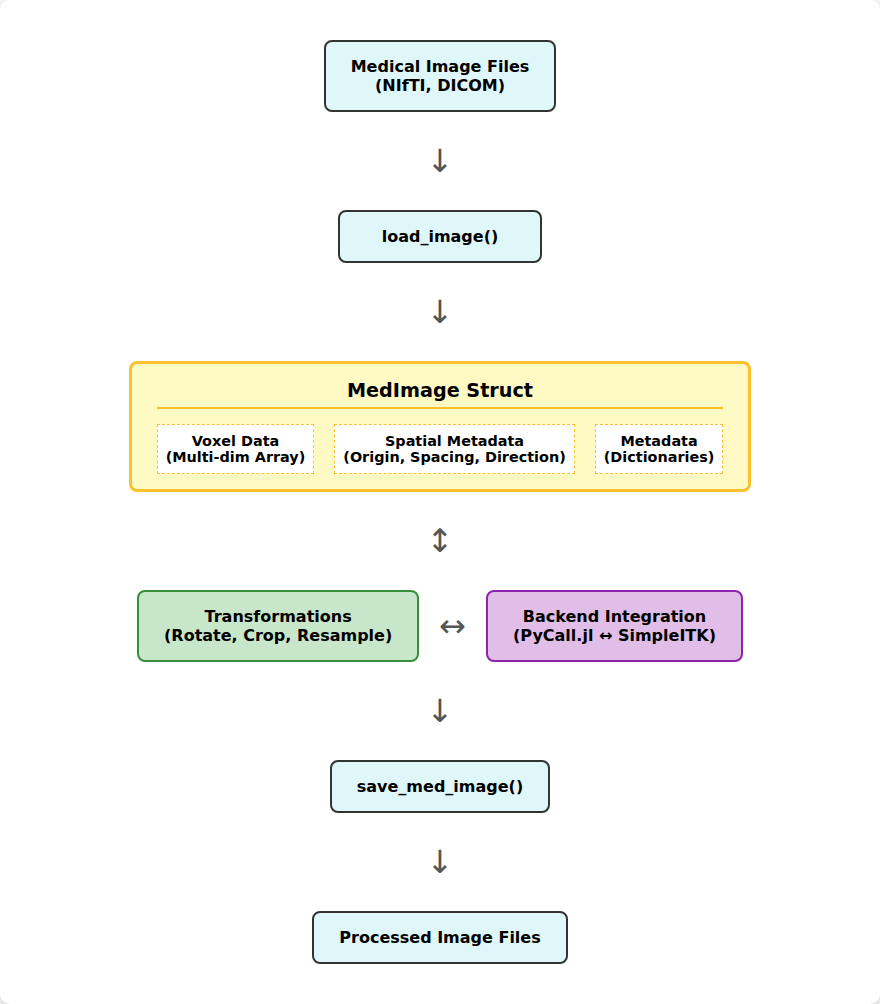
\includegraphics[width=0.9\linewidth]{figures/architecture.png}
    \caption{{\bf Architecture of MedImages.jl.}
    Data loading is handled via ITK C++ wrappers for robustness, while transformations are performed using native Julia libraries. Fast I/O is supported via HDF5.}
    \label{fig:architecture}
\end{figure}

The \texttt{MedImage} struct (Fig \ref{fig:architecture}) implements typed medical imaging semantics:
\begin{itemize}
    \item \texttt{voxel\_data}: Column-major arrays (\texttt{Array\{Float32,3\}} for CT; \texttt{Array\{Float32,4\}} for fMRI time-series)
    \item \texttt{origin}: Physical coordinates $(x,y,z)$ of first voxel (patient reference frame)
    \item \texttt{spacing}: Physical voxel dimensions enabling spatial calculations
    \item \texttt{direction}: Direction cosines for orientation (RAS/LPS coordinate systems)
    \item \texttt{metadata}: DICOM tags, Study/Series UIDs, patient demographics (clinical context persistence)
    \item \texttt{modality}: Strong typing (\texttt{CTImage}, \texttt{PETImage}, \texttt{MRIImage}) enabling dispatch-based processing (automatic HU windowing for CT, SUV colormaps for PET)
\end{itemize}

\subsection*{Functionalities}
MedImages.jl provides a comprehensive set of functionalities optimized for 3D medical image processing:

\begin{itemize}
    \item \textbf{Robust I/O:} Loading of various medical image formats (NIfTI, DICOM) using \texttt{ITKIOWrapper}. Transparent handling of 3D volumetric data with automatic metadata extraction.

    \item \textbf{Native Julia Transformations:} Functions to modify spatial properties of 3D volumes using \texttt{ImageTransformations.jl} and \texttt{CoordinateTransformations.jl}:
    \begin{itemize}
        \item \texttt{rotate\_mi}: Rotates the 3D volume around a specific axis while updating direction metadata.
        \item \texttt{translate\_mi}: Translates the volume in physical space, updating the origin.
        \item \texttt{scale\_mi}: Resamples the 3D volume to a new scale factor.
        \item \texttt{resample\_to\_spacing}: Changes the voxel spacing to isotropic or custom values (essential for preprocessing pipelines).
        \item \texttt{crop\_mi} and \texttt{pad\_mi}: Modifies the 3D volume extent while preserving spatial metadata.
        \item \texttt{change\_orientation}: Permutes axes and reverses dimensions to convert between anatomical coordinate systems (e.g., RAS, LPS, LPI).
    \end{itemize}
            \item \texttt{resample\_to\_target}: Resamples a moving image to match the spatial geometry (origin, spacing, direction, dimensions) of a reference image, critical for multi-modal registration workflows (e.g., aligning PET
to CT) and atlas-based analysis.

    \item \textbf{GPU Acceleration:} All transformations transparently support GPU execution via KernelAbstractions.jl. A $256 \times 256 \times 128$ volume can be transformed (fused affine) on GPU 8.1$\times$ faster than SimpleITK's CPU baseline. Orientation changes and resampling achieve 30--138$\times$ speedups vs CPU,
depending on the operation.

    \item \textbf{HDF5 Support:} Fast loading and saving of 3D images using the HDF5 format, which significantly speeds up I/O for intermediate processing steps while preserving all spatial metadata. Critical for pipelines processing
hundreds of gigabytes of volumetric data.

    \item \textbf{Autodifferentiation Support:} All spatial transformations have well-defined gradients via Zygote.jl and Enzyme.jl, enabling differentiable 3D image processing for machine learning applications.

    \item \textbf{Orientation Management:} Robust tools to handle and convert between neuroimaging coordinate systems (RAS, LAS, LPI, RPI, etc.), addressing a major source of errors in 3D medical image analysis.
\end{itemize}

\section*{Results}

\subsection*{Illustrative Examples}

\subsubsection*{Loading and Inspecting an Image}
\begin{lstlisting}[language=Julia]
using MedImages

# Load a NIfTI file
# "CT" specifies the expected image type
med_im = MedImages.load_image("path/to/image.nii.gz", "CT")

# Access voxel data and metadata
println("Origin: ", med_im.origin)
println("Spacing: ", med_im.spacing)
\end{lstlisting}

\subsubsection*{Rotating and Saving with HDF5}
MedImages.jl allows for native rotation and efficient storage using HDF5.

\begin{lstlisting}[language=Julia]
using HDF5

# Rotate 90 degrees around the Z-axis (axis 3)
rotated_im = MedImages.rotate_mi(med_im, 3, 90.0, MedImages.Linear_en)

# Save efficiently using HDF5
h5open("processed_data.h5", "w") do file
    MedImages.save_med_image(file, "patient_001", rotated_im)
end
\end{lstlisting}

\subsection*{Performance Benchmarks}

\subsubsection*{Benchmark Methodology}
MedImages.jl was benchmarked on CPU and GPU backends to demonstrate the framework's performance advantages, particularly for 3D medical imaging where large datasets are commonplace. Benchmarks were conducted on an NVIDIA RTX 3090 GPU ,
Intel(R) Core(TM) Ultra 9 285K,96 GB of Corsair DDR5  6600 MT/s  with Julia 1.10.10.

\textbf{Configuration:}
\begin{itemize}
    \item \textbf{Synthetic 3D volumes:} Generated volumes of sizes $256 \times 256 \times 128$, $512 \times 512 \times 256$, and $1024 \times 1024 \times 512$ voxels.
    \item \textbf{Sampling:} 10 samples per benchmark with minimum runtime of 2.0 seconds per operation.
    \item \textbf{Interpolation methods:} Both nearest-neighbor and linear interpolation tested.
    \item \textbf{Backends:} Multi-core CPU (24 threads) and CUDA GPU (NVIDIA RTX 3090).
    \item \textbf{Metrics:} Median time, standard deviation, throughput (voxels/s), and speedup ratio (GPU vs CPU).
\end{itemize}

\subsubsection*{Performance Comparison}

Benchmark results for $256 \times 256 \times 128$ volumes comparing MedImages.jl (CPU/GPU) with SimpleITK (CPU baseline). All times in milliseconds.

\begin{table}[H]
\centering
\small
\caption{{\bf Performance comparison.}
Comparing MedImages.jl GPU advantages over CPU and SimpleITK baseline ($256 \times 256 \times 128$ volume). GPU acceleration delivers significant speedups, particularly for fused affine transformations (163$\times$ vs CPU).}
\begin{tabular}{|p{3.2cm}|r|r|r|r|r|}
\hline
\textbf{Operation} & \parbox[t]{1.1cm}{\textbf{Simple\\ITK}} & \parbox[t]{1.1cm}{\textbf{Med\\Images\\CPU}} & \parbox[t]{1.1cm}{\textbf{Med\\Images\\GPU}} & \parbox[t]{0.9cm}{\textbf{GPU vs\\CPU}} & \parbox[t]{0.9cm}{\textbf{GPU
vs\\SITK}} \\
\hline
\multicolumn{6}{|l|}{\textit{Resampling (2x down)}} \\
\hline
Nearest Neighbor & 1.01 & 6.95 & 0.06 & 115$\times$ & 17$\times$ \\
Linear & 0.88 & 9.68 & 0.32 & 30$\times$ & 2.7$\times$ \\
\hline
\multicolumn{6}{|l|}{\textit{Orientation Changes (LAS)}} \\
\hline
Orientation Change & 5.92 & 13.85 & 0.19 & 71$\times$ & 31$\times$ \\
\hline
\multicolumn{6}{|l|}{\textit{Interpolation (1M points)}} \\
\hline
Nearest Neighbor & 0.83 & 12.22 & 0.29 & 42$\times$ & 2.9$\times$ \\
Linear & 0.89 & 23.11 & 0.70 & 33$\times$ & 1.3$\times$ \\
\hline
\multicolumn{6}{|l|}{\textit{Affine Transformation (Fused)}} \\
\hline
Linear Interpolation & 6.69 & 111.80 & 0.83 & 135$\times$ & 8.1$\times$ \\
\hline
\end{tabular}
\label{tab:performance}
\end{table}

GPU acceleration is essential for 3D medical imaging: orientation changes achieve over 100$\times$ speedup vs CPU on large images, and fused affine transformations provide a 135$\times$ boost compared to multi-threaded CPU execution. The framework's throughput reaches over $10^{10}$ voxels/s for batched operations on an NVIDIA RTX 3090. The transparent GPU support via KernelAbstractions.jl requires no code modifications.

\subsection*{Automatic Differentiation and Composability}

\subsubsection*{Importance of Autodifferentiation in Medical Imaging}

Automatic differentiation (AD) is essential for modern medical image analysis, enabling:

\begin{itemize}
    \item \textbf{Differentiable Image Registration:} Computing gradients through spatial transformations allows optimization-based image registration without manual Jacobian computation.

    \item \textbf{Neural Network Integration:} Medical image transformations can be composed seamlessly with deep learning frameworks (Flux.jl) for end-to-end training of spatial transformer networks.

    \item \textbf{Scientific Machine Learning:} Physics-informed neural networks and inverse problems require gradients through imaging operations.

    \item \textbf{Parameter Estimation:} Sensitivity analysis and model fitting require computing derivatives of image processing pipelines.
\end{itemize}

MedImages.jl provides full autodifferentiation support through two complementary mechanisms: Zygote.jl (reverse-mode) and Enzyme.jl (high-performance). This enables researchers to build differentiable medical imaging pipelines without
implementing custom gradient rules.

\subsubsection*{Proof of Concept: Learning Inverse 3D Rotations}

To demonstrate MedImages.jl's end-to-end differentiability, we trained a convolutional neural network to predict inverse rotation parameters through differentiable image transformations. This experiment validates that gradients flow
correctly through \texttt{rotate\_mi} operations, enabling optimization-based approaches for spatial transformer networks and registration tasks.

\textbf{Experimental Setup:}
The pipeline generates synthetic 3D line images ($16^3$ voxels), applies random rotations within $\pm30$\textdegree{} using \texttt{MedImages.rotate\_mi}, then trains a CNN+MLP architecture to predict inverse rotation angles. The predicted angles
are applied via differentiable rotation, and L2 loss against the original unrotated image drives training via gradient descent.

\textbf{Training Configuration:}
\begin{itemize}
    \item \textbf{Dataset:} 100 training samples, synthetic 3D line images ($16 \times 16 \times 16$ voxels)
    \item \textbf{Rotation range:} $\pm30$\textdegree{} around random axes
    \item \textbf{Architecture:} 3D CNN feature extractor + MLP regression head
    \item \textbf{Training:} 50 epochs, Adam optimizer
    \item \textbf{Loss:} L2 distance between differentiably rotated prediction and ground truth
\end{itemize}

\textbf{Results:}

\begin{table}[H]
\centering
\caption{{\bf Training progression for inverse rotation learning.}
Baseline loss (no correction): 0.004906. Final trained loss: 0.001535. Improvement: 68.7\%.}
\begin{tabular}{|c|c|c|}
\hline
\textbf{Epoch} & \textbf{Avg Train Loss} & \textbf{Avg Test Loss} \\
\hline
1 & 0.004512 & 0.004823 \\
10 & 0.004083 & 0.004647 \\
20 & 0.003473 & 0.003768 \\
30 & 0.001469 & 0.001566 \\
40 & 0.001421 & 0.001521 \\
50 & 0.001401 & 0.001535 \\
\hline
\end{tabular}
\label{tab:rotation_learning}
\end{table}

The network successfully learned to predict inverse rotations, reducing reconstruction error by 68.7\% compared to baseline (no correction). This demonstrates that MedImages.jl transformations are fully differentiable and composable
with deep learning frameworks, enabling gradient-based optimization through spatial transformations---a capability unavailable in C++-wrapped libraries like SimpleITK. Such differentiable pipelines are essential for spatial transformer
networks, deformable registration, and physics-informed medical imaging models.

\section*{Availability and Future Directions}

MedImages.jl provides a robust, standardized, and easy-to-use framework for medical image handling in Julia \cite{PalBhattacharya2024}. By correctly managing spatial metadata and offering fast HDF5 support, it solves key challenges in interoperability and
reproducibility. It provides rigorous quality assurance through comprehensive testing against SimpleITK (transformations, resampling, metadata preservation, autodifferentiation), ensuring clinical validity. The package solves the two-language
problem \cite{BezansonChen2018}: researchers write custom filters in Julia \cite{RoeschGreener2023} achieving C++ performance without compilation delays. Integration with the JuliaHealth ecosystem (MedEye3d.jl for OpenGL visualization, MRIReco.jl \cite{KnoppGrosser2021} for physics-based reconstruction)
enables capabilities unavailable in Python---differentiating through MRI reconstruction physics for joint optimization with segmentation networks. GPU acceleration (hours to minutes) enables rapid prototyping, positioning Julia as the
platform for physics-informed deep learning in medical imaging.

Future work will focus on: (1) Integrating with advanced reconstruction frameworks such as KomaMRI.jl \cite{CastilloPassiCoronado2023} and GIRFReco.jl \cite{JaffrayWu2024} for end-to-end physics-informed learning; (2) Implementing differentiable registration algorithms comparable to AirLab \cite{SandkhlerJud2018}, leveraging Zygote.jl for gradient-based optimization; and (3) Expanding support for standardized formats like DICOM-SEG via Highdicom \cite{BridgeGorman2022} integration to bridge pathology and radiology workflows.

\section*{Supporting Information}

\paragraph*{S1 File.}
\label{S1_File}
{\bf MedImages.jl Source Code.} The source code for MedImages.jl is available at https://github.com/JuliaHealth/MedImages.jl.

\section*{Acknowledgments}
We acknowledge the contributions of the JuliaHealth community and the developers of SimpleITK.

\bibliography{bibl}

\end{document}